\documentclass{exam}

\usepackage{amsmath,amssymb,amsfonts}
\usepackage{graphicx}
\usepackage{amsthm}
\usepackage[french]{babel}
\usepackage{enumitem}

\setlength{\topmargin}{-.5in} \setlength{\textheight}{9.25in}
\setlength{\oddsidemargin}{0in} \setlength{\textwidth}{6.8in}

\makeatletter
\def\gap#1{%
  \setbox\@tempboxa\hbox{{\color{white}#1}}%
  \@tempdima\wd\@tempboxa
  \rlap{\unhbox\@tempboxa}%
  \hb@xt@\@tempdima{\dotfill}%
}
\makeatother   

\theoremstyle{definition}
\newtheorem{exercice}{Exercice}

\begin{document}
\Large

\noindent{\bf Contrôle 1 (B) -- 1h. \hfill Première générale -- Groupe 2 \hfill 06/11/2024}
%\vspace{5mm}
%\noindent{\makebox[\textwidth]{Nom et prénom:\enspace\hrulefill}}

%\begin{center}
%\fbox{\fbox{\parbox{5.5in}{\centering
%Répondez dans les espaces fournis. Si vous n'avez plus de place, continuez sur le verso.}}}
%\end{center}

~\\



\medskip\hrule

\begin{exercice}[20 min, 6 points]
    \begin{enumerate}
        \item Pour chacune des suites suivantes, indiquer si elle est arithmétique ou géométrique, et préciser pourquoi. Justifier si elle ne l’est pas.
        \begin{enumerate}
            %\item $u_0 = 2, u_{n+1} = \frac{4 u_n}{3}$.
            \item $u_n = 1.5 \times (\frac{2}{3})^n$.
            %\item $u_1 = 2, u_{n+1} = u_n + \frac{5}{3}$.
            \item $u_n = n^2 - 8n$.
            \item $u_n = 7 - \pi n$.
            \item $u_0 = 1, u_{n+1} = 3nu_n$.
        \end{enumerate}
        \item Pour chaque suite, déterminer ses variations (croissante, décroissante) sur $\mathbb{N}$.
        \item Lorsque c'est possible, exprimer chaque suite de manière explicite et calculer son $100$-ième terme.
    \end{enumerate}
\end{exercice}

\vfill

\begin{exercice}[10 min, 4 points]
\begin{enumerate}
    \item Calculer les sommes suivantes:
    \begin{enumerate}
        %\item $1+\frac{1}{5}+\frac{1}{25}+\dots+\frac{1}{15625}$.
        \item $5+9+13+\dots+493$.
        \item $\frac{4}{3}+\frac{4}{9}+\frac{4}{27}+\dots+\frac{4}{6561}$.
    \end{enumerate}
    \item Exprimer la somme $\sum_{k=2}^{10}(6k+2)$ sous la forme $a+b+\dots+c$.
\end{enumerate}

\vfill
    
\end{exercice}

\begin{exercice}[10 min, 4 points]
    \begin{enumerate}
        \item Dans chaque cas, on donne deux termes d’une suite arithmétique ou géométrique $(u_n)$. Déterminer la raison et le premier terme $(u_0)$ de cette suite.
        \begin{enumerate}
            \item $(u_n)$ est géométrique, $u_3 = 27$ et $u_{6} = 729$.
            \item $(u_n)$ est arithmétique, $u_7 = 31$ et $u_{20} = 45$.
        \end{enumerate}
    \end{enumerate}
\end{exercice}

\newpage
\begin{exercice}[20 min, 6 points]
    On souhaite construire un château de cartes de la manière suivante:
    pour construire un étage, on aligne des groupes de 3 cartes disposés en triangles sur l'étage précédent.
    \begin{center}
        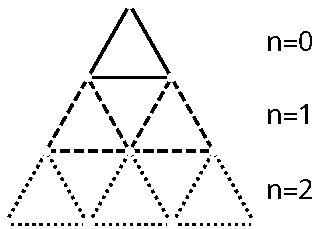
\includegraphics[width=0.5\linewidth]{triangles.pdf}
    \end{center}
    \begin{enumerate}
        \item En numérotant les étages de haut en bas à partir de $0$, soit $u_n$ le nombre de cartes à l'étage $n$, avec $u_0 = 3$.
        \begin{enumerate}
            %\item Donner $u_1$ et $u_2$.
            \item Déterminer l'expression de $u_n$.
        \end{enumerate}

        \item On cherche à calculer le nombre de total cartes $s_n$ présentes dans un château ayant $n$ étages.
        \begin{enumerate}
            \item Donner $s_0$ et $s_1$.% et $s_2$.
            \item Déterminer l'expression de $s_n$.
        \end{enumerate}

        \item On dispose de 315 cartes. Combien d'étages peut-on construire ?
    \end{enumerate}
\end{exercice}

\end{document} 
\begin{exercice}[Calculer]
    \begin{enumerate}
        \item Pour chacune des suites suivantes. Dire si elle est arithmétique, géométrique ou non.
        \begin{enumerate}
            \item $u_1 = 1, u_{n+1} = u_n + \frac{7}{4}$.
            \item $u_0 = 1, u_{n+1} = \frac{3 u_n}{2}$.
            \item $u_0 = 1, u_{n+1} = 2nu_n$.
            \item $u_n = 5 - \pi n$.
            \item $u_n = n^2$.
            \item $u_n = 2.3 \times (\frac{1}{2})^n$.
            \item $u_n = n^2 - 10n$.
        \end{enumerate}
        \item Pour chaque suite, déterminez ses variations (croissante, décroissante) sur $\mathbb{N}$.
        \item Pour chaque suite, lorsque c'est possible, calculez son $100$-ième terme.
    \end{enumerate}
\end{exercice}

\begin{exercice}[Calculer]
\begin{enumerate}
    \item Calculez les sommes suivantes:
    \begin{enumerate}
        \item $3+7+11+\dots+487$.
        \item $1+\frac{1}{4}+\frac{1}{16}+\dots+\frac{1}{16384}$.
        \item $\frac{2}{3}+\frac{2}{9}+\frac{2}{27}+\dots+\frac{2}{2187}$.
    \end{enumerate}
    \item Exprimez la somme $\sum_{k=2}^{10}(5k+1)$ sous la forme $a+b+\dots+c$.
\end{enumerate}
    
\end{exercice}

\begin{exercice}[Modéliser]
    \begin{enumerate}
        \item Dans chaque cas, on donne deux termes d’une suite arithmétique ou géométrique $(u_n)$. Déterminer le premier la raison et le premier terme $(u_0)$ de cette suite.
        \begin{enumerate}
            \item $(u_n)$ arithmétique, $u_7 = 31$ et $u_{20} = 45$.
            \item $(u_n)$ géométrique, $u_3 = 27$ et $u_{6} = 729$.
        \end{enumerate}
    \end{enumerate}
\end{exercice}

\newpage
\begin{exercice}
    Pierre-Alexandre construit un château de cartes de la manière suivante.
    Pour construire un étage il aligne des groupes de 3 cartes disposés en triangle sur l'étage précédent.
    \begin{enumerate}
        \item En numérotant les étages de haut en bas à partir de $0$. Soit $u_n$ le nombre de cartes à l'étage $n$, ainsi $u_0 = 3$.
        \begin{enumerate}
            \item Donner $u_1, u_2$.
            \item Donner l'expression de $u_n$.
        \end{enumerate}

        \item On cherche à calculer le nombre de cartes $s_n$ présent dans un château à $n$ étages.
        \begin{enumerate}
            \item Donner $s_0$, $s_1$, $s_2$.
            \item Donner l'expression de $s_n$.
        \end{enumerate}

        \item Pierre-Alexandre dispose de 1340 cartes. Combien pourra t'il construire d'étages ?
    \end{enumerate}
\end{exercice}

\end{document} 

\end{document} 